\chapter{Theoretical background}

This chapter will cover the necessary theory used to formulate and solver our problem. Main focus will be on graph topology and alternative graphs and their relation to the train dispatching problem. 

\section{Basic definitions}
While some of these definitions may feel redundant, we will use them as an opportunity to establish the notation. Most of the definitions are paraphrased from \emph{Handbook of Graph Theory} \cite{gross2013handbook} with notation adjusted to ours.


\begin{definition}
Graph is an ordered pair $G = (V,\ E)$, where $V = \{v_i\}_{i=1}^{n_v}$ is a set vertices \footnote{\label{note:nodes}Vertices are often called nodes.} and $E = \{e_i\}_{i=0}^{n_e}$ is a set of edges, where edge $e = \{u,\ v\},\ u,\ v \in V$ is an \emph{unordered} pair of vertices.
\end{definition}

\begin{definition}
\label{def:digraph}
Directed graph (digraph) is an ordered pair $G = (V,\ E)$, where $V = \{v_i\}_{i=1}^{n_v}$ is a set vertices and $E = \{e_i\}_{i=0}^{n_e}$ is a set of edges \footnote{\label{note:arcs}Commonly the edges in directed graphs are called arcs.}, where edge $e = (u,\ v),\ u,\ v \in V$ is an \emph{ordered} pair of vertices.
\end{definition}


\begin{definition}
Multigraph is an ordered tuple $G = (V,\ E,\ r)$, where $V = \{v_i\}_{i=1}^{n_v}$ is a set vertices, $E = \{e_i\}_{i=0}^{n_e}$ is a set of edges and $r:\ E \rightarrow \{\{u,\ v\}\ |\ u,\ v \in V\}$ is a mapping from edges to pair of endpoint vertices.
\end{definition}

\begin{definition}
Directed multigraph is an ordered tuple $G = (V,\ E,\ s,\ t)$, where $V = \{v_i\}_{i=1}^{n_v}$ is a set vertices, $E = \{e_i\}_{i=0}^{n_e}$ is a set of edges and $s:\ E \rightarrow V$ is a source (start) mapping from edges to vertices and $t:\ E \rightarrow V$ is a target (end) mapping from edges to vertices.
\end{definition}


Example of each type of graph is in figure \ref{fig:graph_example}.

\begin{remark}
As you can see in figure \ref{fig:graph_example}, digraph allows for parallel edges (2, 3) and (3, 2). This will be a useful property for the alternative graph definition.
\end{remark}

\begin{figure}[htbp!]
\caption{Example of graph (A), digraph (B), multigraph (C) and directed multigraph (D)}
\label{fig:graph_example}
\begin{center}
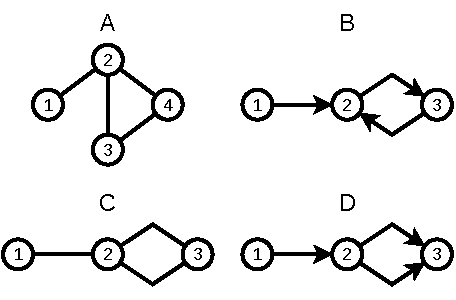
\includegraphics[width=.8\textwidth]{img/graph_example.pdf}
\end{center}
\end{figure}

Since we will mostly be working with directed graph, to following definitions are tailored for directed graphs. The following definitions of operators also abuse the notation by ommiting the specification of graph $G$, which will be included in the context of multiple graphs if necessary.

\begin{definition}
Source (start) $\src(e) = u,\ e = (u,\ v)$ is the starting vertex of edge $e$.
\end{definition}

\begin{definition}
Target (end) $\tar(e) = v,\ e = (u,\ v)$ is the ending vertex of edge $e$.
\end{definition}

\begin{definition}
Incomming edges $\inedges(v) = \{e\ |\ t(e) = v,\ e \in E\}$ of vertex $v$ is a set of edges $e$ that end in $v$.
\end{definition}

\begin{definition}
Outgoing edges $\outedges(v) = \{e\ |\ s(e) = v,\ e \in E\}$ of vertex $v$ is a set of edges $e$ that start in $v$.
\end{definition}

\begin{definition}
Predecessors (In-neighborhood) $\inver(v) = \{u\ |\ u = \src(e),\ e \in \inedges(v)\}$ of vertex $v$ is a set of vertices $u$ that are connect to $v$ via its incomming edges.
\end{definition}

\begin{definition}
Successors (Out-neighborhood) $\outver(v) = \{w\ |\ w = \tar(e),\ e \in \outedges(v)\}$ of vertex $v$ is a set of vertices $w$ that are connect to $v$ via its outgoing edges.
\end{definition}

\begin{definition}
In-degree $\indeg(v) = |\inedges(v)|$ is the number of incomming edges of $v$.
\end{definition}

\begin{definition}
Out-degree $\outdeg(v) = |\outedges(v)|$ is the number of incomming edges of $v$.
\end{definition}

\begin{definition}
Path is $P = \mathrm{P}(u,\ v)$ from $u$ to $v$ is a sequence of edges $(e_i)_{i=1}^N$, such that $\tar(e_{i-1}) = \src(e_i),\ 2 \leq i \leq n$, $u = src(e_0)$ and $v = \tar(e_n)$.
\end{definition}

\begin{definition}
Cycle is a path that starts and ends in the same vertex.
\end{definition}

\section{Graph topology}
\begin{definition}
Directed acyclic graph (DAG) is directed graph that contains no cycle.
\end{definition}

\begin{definition}
Topological order is a sequence of vertices in directed graph $(v_i)_{i=1}^{|V|}$ such that $e = (u, v) \implies u \prec v$ ($u$ apears before $v$ in the sequence).
\end{definition}

\begin{theorem}
Topological order can only be created for acyclic graphs.
\end{theorem}

\begin{proof}
By contradiction, for path starting at $u$ and ending at $v$, $u \prec v$ in the topological order, because for each $e = (x, y)$ in path, $x \prec y$ and ordering $\prec$ is transitive. For cycle $u$ and $v$ are in the same spot in the order, this is a contradiction.
\end{proof}

To detect a cycle and get a topological sort we use algorithm \ref{alg:toposort}, it is acombination for depths first search (DFS) for cycle detection and DFS for topological sorting \cite{CLRS2022}. It runs in $\mathrm{O}(|V| + |E|)$ time complexity with $\mathrm{O}(|V|)$ required space. It allows us to do both cycle detection and topological sort in one pass of DFS.

\begin{algorithm}[float, caption={Topological sort with cycle detection}, label={alg:toposort}]
input: graph G
output: () if G contains cycle else topological order of G

function: DFS(v, label, stack)
  if label(v) is InRecursion
    return true
  else if label(v) is Done
    return false
  end

  label(v) $\gets$ InRecursion

  foreach s $\in \outver$(v)
    if DFS(s, label, stack)
      return true
    end
  end

  stack.push(v)
  label(v) $\gets$ Done

  return false
end

begin
  foreach v $\in$ V(G)
    label(v) $\gets$ NotDone
  end

  stack $\gets$ EmptyStack

  foreach v $\in$ V(G)
    if DFS(v, label, stack)
      return ()
    end
  end

  order $\gets$ reverse(stack)
  return order
end
\end{algorithm}


\section{Alternative graphs}

Alternative graphs were introduced in \cite{MASCIS2002498}. The provide a very useful framework for modeling resource allocation problems with blocking. They are a generalization of disjunctive graphs \cite{roy1964problemes}.

\begin{definition}
Alternative graph is an ordered tuple $G = (V,\ E,\ A)$, where $V = \{v_i\}_{i=1}^{n_v}$ is a set vertices, $E = \{e_i\}_{i=0}^{n_e}$ is a set edges $e = (u,\ v),\ u,\ v \in V$, and $A = \{a_i\}_{i=0}^{n_a}$ is a set of disjunctive (alternative) edge pairs $a = ((u,\ v),\ (x,\ y)),\ u,\ v,\ x,\ y \in V$.
\end{definition}

\begin{remark}
We denote the alternative $\bar{e}$ to the edge $e$ from the disjunctive pair $a = (e,\ \bar{e})$.
\end{remark}

To illustrate the concept of alternative graphs, figure \ref{fig:alt_graph_example} shows an altertative graph with 3 disjunctive pairs.

\begin{figure}[htbp!]
\caption{Example of alternative graph}
\label{fig:alt_graph_example}
\begin{center}
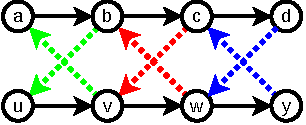
\includegraphics[width=0.6\textwidth]{img/alt_graph_example.pdf}
\end{center}
\end{figure}

\begin{definition}
A selection $S$ is a set of edges obtained by from $A$ by choosing at most one edge from each pair. The edges in this selection are selected, their alternatives (the other edge from the pair) is forbidden. 
\end{definition}

\begin{definition}
Selection $S$ is complete if exactly one edges is chosen from each pair, otherwise its a partial selection. 
\end{definition}

\begin{definition}
Selection $S$ is consistent if graph $(V,\, E \cup S)$ does not contain a cycle. If the graph does contain a cycle, the selection is inconsistent.
\end{definition}

To illustrate the selection terms, figure \ref{fig:alt_graph_selection} shows different types of selections from on alternative graph from figure \ref{fig:alt_graph_example}.

\begin{figure}[htbp!]
\caption{Examples for partial inconsistent (A), partial consistent (B), complete inconsistent (C), and complete consistent (D) selections}
\label{fig:alt_graph_selection}
\begin{center}
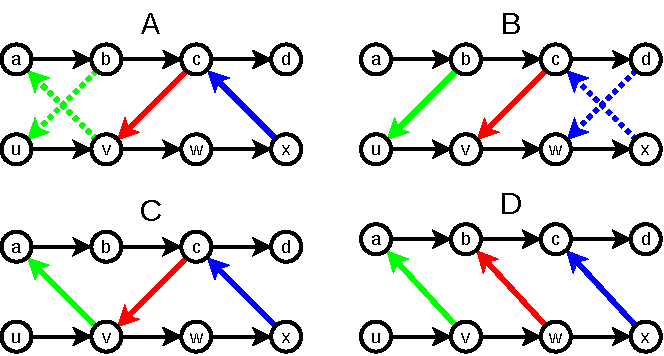
\includegraphics[width=1.0\textwidth]{img/alt_graph_selection.pdf}
\end{center}
\end{figure}

\begin{definition}
Alternative edge $e$ is inferred from selection $S$, $S \vdash e$ if $S \cup \{\bar{e}\}$ is an inconsistent selection, meaning that the choice of $e$ from altertative pair $(e,\ \bar{e})$ can be inferred from $S$ because choosing $\bar{e}$ would be inconsistent. Similarly we can say that one alternative edge $x$ implies another $y$, $x \implies y$ if $\{x\} \vdash y$.
\end{definition}


An example from on graphs in figure \ref{fig:alt_graph_example}, we can see that $(b,\ u) \implies (c,\ v)$ and $(v,\ a) \implies (w,\ b)$ etc.

\begin{remark}
It is possible to have a partial consistent selection $P$ for which there exist no complete consistent complete selection $C$, $P \subset C$. One such case is in figure \ref{fig:alt_graph_infeasible}, where $(b,\ u) \implies (c,\ v)$ and $(x,\ c) \implies (w,\ b)$. Beacuse $(c,\ v)$ and $(w,\ b)$ are in the same disjunctive pair, we cannot make a consistent selection for this pair.
\end{remark}


\begin{figure}[htbp!]
\caption{Examples of partial consistent selection without possible complete consistent selection}
\label{fig:alt_graph_infeasible}
\begin{center}
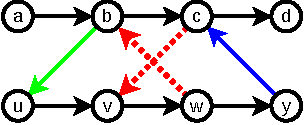
\includegraphics[width=.6\textwidth]{img/alt_graph_infeasible.pdf}
\end{center}
\end{figure}

\subsection{Weighted graphs}

To extend the descriptive ability of graphs to model problems we assign properties to vertices or edges. One of the most common one is to add weights to edges.

\begin{definition}
Weighted directed graph is an ordered tuple $G = (V,\ E,\ w)$, where $V$ and $E$ are same as in digraph definition \ref{def:digraph}, and $w: E \rightarrow \mathbb{R}$ is an edge weight mapping.
\end{definition}


\begin{definition}
Length $\mathrm{L}(\cdot)$ of path $P$ is the sum of the weights for each edge,
\begin{equation}
\mathrm{L}(P) = \sum_{e \in P} w_e
\end{equation}
\end{definition}


\begin{definition}
Length of the longest path $\mathrm{L_{max}}(\cdot)$ from $u$ to $v$ is
\begin{equation}
	\mathrm{L_{max}}(u, v) = \max_{P \in \mathcal{P}_{u,v}}\mathrm{L}(P),
\end{equation}
where $\mathcal{P}_{u,v}$ is the set of all paths from $u$ to $v$.
\end{definition}

\begin{remark}
Length of the longest path can only be calculated for a graph without any positive length cycles, otherwise we could simple go in the cycle indefinitely to prolong the path.
\end{remark}

For our model, the weight of an edge will be coresponding to a minimal duration between events. We can construct an event graph like in figure \ref{fig:event_graph} where each vertex is an event, with origin $o$ as the start and each edges weight defines minimal duration between the events.

\begin{figure}[htbp!]
\caption{Examples of event graph for 3 trains with shared resources}
\label{fig:event_graph}
\begin{center}
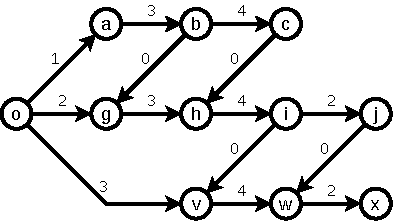
\includegraphics[width=.7\textwidth]{img/event_graph.pdf}
\end{center}
\end{figure}

The time of the event $x$ in the even graph can be calculate as the longest path from origin $o$ to $x$, $\mathrm{T}(x) = \mathrm{L_{max}}(o,\ x)$.


Finding all of the paths from $o$ to each $x \in V$ would be very expensive, by DFS the complexity is exponential \cite{homer2011computability}.

First optimization is the use of Bellman principle \cite{light2024principle}\cite{bellman1952dynamic},

\begin{equation}
	\mathrm{T}(v) = \mathrm{L_{max}}(o,\ v) = \max_{u \in \inver(v)} \mathrm{L_{max}}(o,\ u) + w_{(u,\ v)}.
\end{equation}

This is principle is used by the Floyd-Warshall algorithm \cite{floyd1962algo} and Dijkstra's algorithm \cite{Dijkstra1959} which are used for finding shortest paths for all pairs for vertices and from a select starting vertex respectively. Both of them could be adjusted to find the longest path within polynomial complexity, $\mathrm{O}({|V|}^3)$ for Floyd-Warshall and $\mathrm{O}((|V| + |E|)log|V|)$ for Dijkstra with binary heap.

Since we already use algorithm \ref{alg:toposort} to detect a cycle, we can just process the time of the nodes in the topological order.

\begin{definition}
Critical path $\mathrm{CP}(\cdot)$ for vertex $v$ is the longest path from origin $o$ to $v$.
\end{definition}

Critical path  is limiting the earliest start of event $v$, delaying any event along this path will also delay the event $v$,

\begin{equation}
	\mathrm{L}(\mathrm{CP}(v)) = \mathrm{T}(v).
\end{equation}

\begin{definition}
Critical path edge $\mathrm{CPE}(\cdot)$ of $v$ is the last edge of the critical path for $v$.
\end{definition}

We can again use the Bellman principle to reconstruct the critical path,
\begin{equation}
	\mathrm{CP}(v) = \mathrm{CP}(u) \cup \{(u,\ v)\},\ \mathrm{CPE}(v) = (u,\ v).
\end{equation}

Algorithm \ref{alg:time} outputs the time $\mathrm{T}(\cdot)$ and critical path edge $\mathrm{CPE}(\cdot)$ for each vertex in the event graph. It runs in $\mathrm{O}(|V| + |E|)$ time complexity.

\begin{remark}
In our event graph, the first vertex in the topological order will always be the origin $o$ as it is the only vertex $v$ with $\indeg(v) = 0$.
\end{remark}

\begin{algorithm}[float, caption={Time and critical path predecessor calculation}, label={alg:time}]
input: weighted graph G, topological order O
output: time T and critical path edge CPE for each vertex in G

begin
  foreach v $\in$ V(G)
    T(v) $\gets$ 0
    CPE(v) $\gets$ Undefined
  end

  foreach u $\in$ O $\setminus$ {o}
    foreach (u, v) $\in \outedges$(u)
      if T(v) < T(u) + w$_{u,v}$
        T(v) $\gets$ T(u) + w$_{u,v}$
        CPE(v) $\gets$ (u, v)
      end
    end
  end
end
\end{algorithm}

\paragraph{Example} For event graph in figure \ref{fig:event_graph}, the time and critical path edge output from algorithm \ref{alg:time} is in table \ref{tab:time_crit}. So the vertices in the critical path for $a$ are ($o$, $a$, $b$, $c$), for $j$ are ($o$, $a$, $b$, $c$, $h$, $i$, $j$) and for $w$ are ($o$, $a$, $b$, $c$, $h$, $i$, $u$, $v$, $w$).

\begin{table}[htbp!]
\begin{center}
\caption{Time and critical path edge for vertices in example from figure \ref{fig:event_graph}}\label{tab:time_crit}
\begin{tabular}{lrc}
\toprule
vertex & T & CPE \\
\midrule
a & 1 & (o, a) \\
b & 4 & (a, b) \\
c & 8 & (b, c) \\
g & 4 & (b, g) \\
h & 8 & (c, h) \\
i & 12 & (h, i) \\
j & 14 & (i, j) \\
u & 12 & (i, u) \\
v & 16 & (u, v) \\
w & 18 & (v, w) \\
\bottomrule
\end{tabular}
\end{center}
\end{table}
